\documentclass[14pt,class=minimal,border=5pt]{standalone}

\usepackage{amsmath}
%\usepackage{amsthm}
\usepackage{amssymb}
\usepackage{graphicx}


\usepackage[scaled]{helvet}
\renewcommand\familydefault{\sfdefault} 
\usepackage[T1]{fontenc}



\usepackage{mathrsfs} % mathscr fonts

%\usepackage{setspace}

\usepackage{tikz}
\usetikzlibrary{trees,positioning,arrows,matrix}
\usetikzlibrary{decorations.pathmorphing,decorations.pathreplacing}
\usetikzlibrary{calc}

\usepackage{scalefnt}


%\usepackage[active,tightpage]{preview}
%\PreviewEnvironment{tikzpicture}

%\setlength\PreviewBorder{5pt}%


\newcommand{\pd}[2]{\frac{\partial #1}{\partial #2}}
\newcommand{\pdm}[3]{\frac{\partial^{#3} #1}{\partial #2^{#3}}}
\newcommand{\od}[2]{\frac{\mathrm{d} #1}{\mathrm{d} #2}}
\newcommand{\odm}[3]{\frac{\mathrm{d}^{#3} #1}{\mathrm{d} #2^{#3}}}
\newcommand{\dx}[1]{\ \mathrm{d} #1}
\newcommand{\E}{\mathbb{E}}
\newcommand{\Var}{\text{Var}}
\renewcommand{\Re}{\text{Re}}
\renewcommand{\Im}{\text{Im}}
\newcommand{\half}{\frac{1}{2}}

\newcommand{\btheta}{\boldsymbol{\theta}}
\newcommand{\Y}{\mathbf{Y}}
\newcommand{\Z}{\mathbf{Z}}
\newcommand{\C}{\mathbf{C}}
\newcommand{\z}{\mathbf{z}}
\newcommand{\xmin}{x_\mathrm{min}}
\newcommand{\argmax}[1]{\underset{#1}{\operatorname{argmax}}\ }
\newcommand{\bphi}{\boldsymbol\phi}



\makeatletter
\let\@currsize\normalsize
\makeatother

%\def\w{20cm}
%\def\h{14cm}
\def\x{0}
\def\y{0}


\begin{document}

  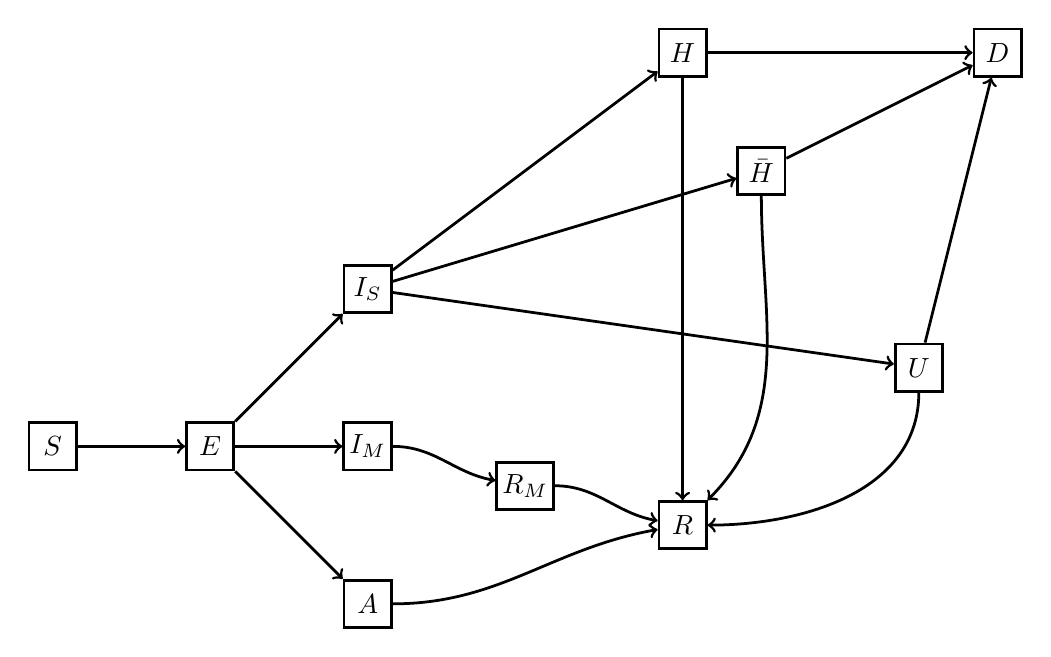
\begin{tikzpicture}[minimum size=6mm,inner sep=2pt,line width=1pt,decoration={random steps,segment length=2pt,amplitude=1.5pt}]
%\begin{tikzpicture}
%\coordinate (a) at (0,0);
%\coordinate (b) at (2,2);
%\draw (a) -- (b);


\node[shape=rectangle, draw=black] (S) at (0,0) {$S$};
\node[shape=rectangle, draw=black] (E) at (2,0) {$E$};
\node[shape=rectangle, draw=black] (Im) at (4,0) {$I_M$};
\node[shape=rectangle, draw=black] (Is) at (4,2) {$I_S$};
\node[shape=rectangle, draw=black] (A) at (4,-2) {$A$};

\node[shape=rectangle, draw=black] (Rm) at (6,-0.5) {$R_M$};

\node[shape=rectangle, draw=black] (R) at (8,-1) {$R$};

%\node[shape=circle, draw=black, scale=0.15] (Hstream) at (6,2.5) {};
\node[shape=rectangle, draw=black] (H) at (8,5) {$H$};
\node[shape=rectangle, draw=black] (Hbar) at (9,3.5) {$\bar{H}$};
\node[shape=rectangle, draw=black] (U) at (11,1) {$U$};

\node[shape=rectangle, draw=black] (D) at (12, 5) {$D$};

%\node[shape=circle, draw=black, scale=0.15] (outH) at (8,4) {};
%\node[shape=circle, draw=black, scale=0.15] (outHbar) at (10,2.5) {};
%\node[shape=circle, draw=black, scale=0.15] (noHstream) at (6,1.5) {};


\path [->] (S) edge node {} (E);
\path [->] (E) edge node {} (Im);
\path [->] (E) edge node {} (Is);
\path [->] (E) edge node {} (A);
%\path [->] (Im) edge node {} (R);
\draw [->] (Im) to [out=0, in=170] (Rm);
\draw [->] (Rm) to [out=0, in=170] (R);
\draw [->] (A) to [out=0, in=190] (R);
%\path [->] (A) edge node {} (R);

%\path [-] (Is) edge node {} (Hstream);
%\path [->] (Hstream) edge node {} (H);
%\path [->] (Hstream) edge node {} (Hbar);

\path [->] (Is) edge node {} (H);
\path [->] (Is) edge node {} (Hbar);
\path [->] (Is) edge node {} (U);

\path [->] (H) edge node {} (D);
\path [->] (Hbar) edge node {} (D);
\path [->] (U) edge node {} (D);


\path [->] (H) edge node {} (R);
\draw [->] (Hbar) to [out=270, in=45] (R);
\draw [->] (U) to [out=270, in=0] (R);

%\path [-] (H) edge node {} (outH);
%\path [->] (outH) edge node {} (R);
%\path [->] (outH) edge node {} (D);
%\path [->] (Hbar) edge node {} (R);
%\path [-] (Hbar) edge node {} (outHbar);
%\draw [->] (outHbar) to [out=270, in=30] (R);
%\path [->] (outHbar) edge node {} (D);

%\path [-] (Is) edge node {} (noHstream);
%\path [->] (noHstream) edge node {} (R);
%\draw [->] (noHstream) to [out=330, in=-90] (D);

 \end{tikzpicture}

\end{document}

